%Un exercice avec son corrigé à inclure dans un fichier principal.

\exo{Donner les ensembles de définition des fonctions suivantes}

\question{}
$f_1(x) = \dfrac{1}{x^2-1}$

\correction{
L'expression de $f_1(x)$ contient une écriture fractionnaire avec $x$ au dénominateur. Il faut donc résoudre l'équation $x^2-1$ pour trouver les potentielles valeurs interdites. 

$x^2 - 1 = 0$

$\Leftrightarrow x^2 = 1$

$\Leftrightarrow x = 1$ ou $x = -1$

L'ensemble de définition est donc: 

\Answer{$D_{f_1} = \mathbb{R} - \{-1 ; 1\}$}
}

\question{}
$f_2(x) = \sqrt{\dfrac{2x-1}{x+4}}$

\correction{
Pour que $f_2(x)$ soit défini, il faut que $\dfrac{2x-1}{x+4} \geqslant 0$

Il faut donc dresser un tableau de signe de $\dfrac{2x-1}{x+4}$. Pour ce faire, il faut d'abord étudier le signe du numérateur et du dénominateur:

\begin{itemize}
 \item $2x-1 \geqslant 0 \Leftrightarrow x \geqslant \frac{1}{2}$
 \item $x+4 \geqslant 0 \Leftrightarrow x \geqslant -4$
\end{itemize}

On peut maintenant dresser le tableau de signe:

\begin{center}
\begin{tikzpicture}
   \tkzTabInit{$x$ / 1 , $2x-1$ / 1 , $x+4$ / 1, $\dfrac{2x-1}{x+4}$ / 1}{$-\infty$, $-4$, $\frac{1}{2}$ , $\infty$}
   \tkzTabLine{, -,  , -,  z,+}
   \tkzTabLine{, -, z, +,   ,+}
   \tkzTabLine{, +, d, -,  z,+}
\end{tikzpicture}
\end{center}

D'où: $\dfrac{2x-1}{x+4} \geqslant 0 \Leftrightarrow x \in ]-\infty ; -4 [ \cup \left[\frac{1}{2} ; +\infty \right]$

On a donc

\Answer{$D_{f_2} = ]-\infty ; -4 [ \cup \left[\dfrac{1}{2} ; +\infty \right[$}
}
